\chapter{Test Results}

To understand how well the trained agent performs, training results are not enough since they only provide information about how well rewarded the agent is, and not about how it will perform in a real environment. For this, several tests were set up for the 3 types of problems that were tackled in this paper.


\section{Reaching a static target} \label{test_reach_static_target}

For reaching a static target, the test consists of an agent that has to touch 40 targets that are static (i. e. not moving) and that appear in a predefined order. Once the agent touches the target, it disappears and a new one appears in a new location, according to the predefined order. For each test, the same predefined order of targets is used so that the test course is the same for each run. 

Initially, this test was done using only agents that were trained to reach static targets, however a more robust experiment would be to also run the test using agents that were trained to reach moving targets, and compare the results at the end.


\subsection{Agent trained to reach static targets}

The results for testing the agent that was trained to reach static targets can be seen in Table \ref{move_to_static_target_test_results:1} and Figure \ref{test_results_static_target_static_brain_bar_chart}. It can be observed that, unlike the training results, using a smaller network architecture does not yield better times, with the architecture with 5 hidden layers and 128 units per layer being the one that achieved the best time, 170.9822 seconds. For the architecure with a single hidden layer, the configuration with 128 units was faster by 22.66 seconds ($11.01\%$) than the one with 512 units per layer. Since the configuration with 256 units per layer was unable to be trained, because it learned just to move in a circle, it was unable to finish the test course.

For the architecture with 3 hidden layers, the results were much more similar, with the configurations that had 256 and 512 units per layer, having virtually identical times, with the difference between them being 0.2 seconds, and the configuration with 128 units being slower than these two by 2 seconds ($\sim1\%$ slower). These results are somewhat surprising since there was a differnce of $29\%$ in the training performance of the configuration with 128 units compared to the one with 512 units.

The architecture with 5 hidden layers has the configuration that is the best performing in this test, the one with 128 units per layer, which manages to achieve a time of 170.9822 seconds. The other two configurations perform worse, the one with 256 units being slower by 15.4805 seconds ($\sim8.3\%$ slower), and the one with 512 units being slower by 34.8443 seconds ($\sim16.92\%$ slower). This shows that a smaller number of layers does not necessarily lead to better results, however, using less units per hidden layer usually means that the agent will perform better.

The final network architecture, the one with 7 layers has the configuration with 256 units be the fastest one in the test, clocking in at 182.1618 seconds. The configuration with 128 units was slower by 5.8818 seconds ($3.22\%$), and the one with 512 units was slower by 37.279 seconds ($20.46\%$).

\paragraph{}
In summary, from this test we can see that increasing the number of hidden layers used in the architecture does not necessarily decrease the agent's performance, when using up to 5 layers. Also, using a smaller number of units per layer tends to lead to better agent performance. This could be due to the fact that, according to \cite{eldan2016powerofdepth}, increasing the width of the network can lead to overfitting.

\begin{table}
    \centering
    \begin{tabular}{|| m{15em} | m{15em} ||}
    \hline \hline
    \strong{Network Configuration} & \strong{Time to complete ($s$)} \\ \hline \hline
    1 layer, 128 units & 183.1415 \\ \hline
    1 layer, 256 units & DNF \\ \hline
    1 layer, 512 units & 205.8087 \\ \hline
    3 layers, 128 units & 182.1884 \\ \hline
    3 layers, 256 units & 180.4801 \\ \hline
    3 layers, 512 units & 180.2796 \\ \hline
    5 layers, 128 units & 170.9822 \\ \hline
    5 layers, 256 units & 186.4627 \\ \hline
    5 layers, 512 units & 205.8265 \\ \hline
    7 layers, 128 units & 188.0436 \\ \hline
    7 layers, 256 units & 182.1618 \\ \hline
    7 layers, 512 units & 219.4408 \\ \hline \hline
    \end{tabular}
    \caption{Test results for reaching a static target using agent that was trained to reach static targets}
    \label{move_to_static_target_test_results:1}
\end{table}

\begin{figure}
    \begin{center}
        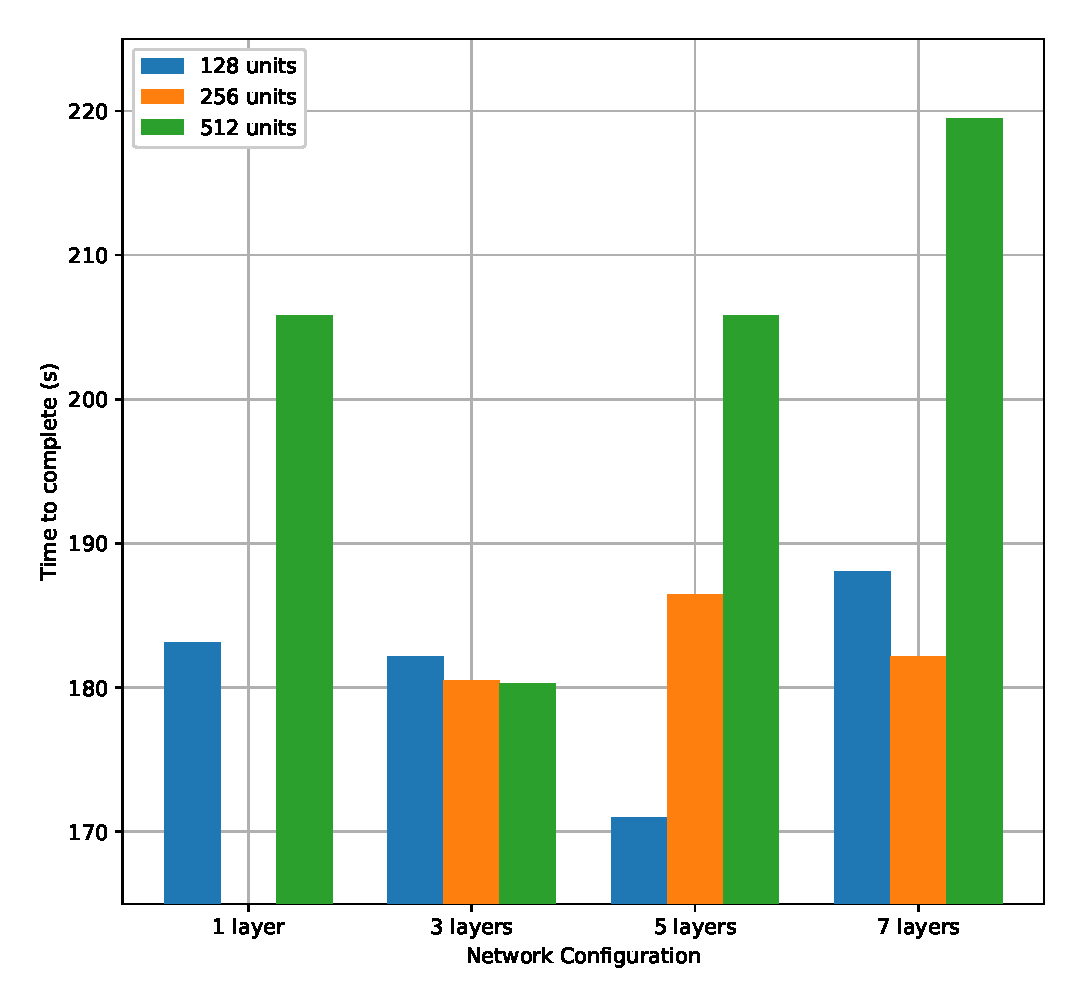
\includegraphics[width=\linewidth]{move_to_static_target_test_static_brain_bar_chart.eps}
        \caption{Test results for reaching a static target using agent that was trained to reach static targets}
        \label{test_results_static_target_static_brain_bar_chart}
    \end{center}
\end{figure}


\subsection{Agent trained to reach moving targets}

The second part of the test is measuring how well an agent that was trained to reach moving targets can also reach static targets, and if it could also beat the agent that was trained to reach static targets. The obtained results are in Table \ref{move_to_static_target_test_results:2} and Figure \ref{test_results_static_target_moving_brain_bar_chart}. Just like in the training Section \ref{moving_target:training}, half of the tested agents will also have the target's direction as an observation (which is the vector $(0, 0, 0)$ since the target is not moving).

Looking at the results for the architecture with just a single hidden layer, it apperas that the best performing configurations are the ones with 128 units per layer, with the one without the target's direction observation being slightly faster, by 3.5389 seconds ($1.8\%$). The configuration with 256 units per layer and with the target's direction observation takes 464.985 seconds to finish the test, more than twice the amount of time it took with 128 units per layer, due to the fact that it becomes stuck trying to move through a narrow path and can't decide to go through, because it tries to find an alternative path that does not exist. For the configurations with 512 units, the one where the target's direction is observed is faster than the other one by 7.2391 seconds ($3.36\%$).

For the architecture with 3 hidden layers, the agents that observed the target's direction were faster than the others that did not. The fastest configuration was the one with 512 units per layer with the time of 188.5515 seconds. The second best was the one with 128 units which was slower by 3.6596 seconds ($1.9\%$). The agents that had 256 and 512 units per layer and did not observe the target's direction, had very slow times, of 491.0297 seconds and 602.9445 seconds respectively. This was due to the fact that the agent became somehow confused and did not manage to get around the level's geometry.

The architecture with 5 hidden layers has both the slowest and fastest configuration, for this type of agent and test, at the same time. The fastest configuration was the one with 128 units and with the target's direction observation, and it finished the test course in 187.1074 seconds. The slowest configuration was the one with 512 units and without the target's direction observation, and it managed to finish the course in 576.1487 seconds. This was due to the fact that the agent was not able to correctly go around a wall and kept trying to go the wrong way for a long period of time. The configuration with 256 units and no target direction observation also managed to score a bad time of 363.128 seconds, becoming stuck in the same place as the previoulsy mentioned one.

In summary, here too, having a smaller number of units per layer seems to increase the performance of the agent, with almost all architectures having their best times be achieved by configurations with 128 units per layer. As for including the target's direction observation, it seems to positively impact the agent only when using a larger number of layers.

\begin{table}
    \centering
    \begin{tabular}{|| m{11.3em} | m{10em} | m{9.6em} ||}
    \hline \hline
    \strong{Network Configuration} & \strong{Observed target's direction} & \strong{Time to complete ($s$)} \\ \hline \hline
    1 layer, 128 units & No & 192.7527 \\ \hline
    1 layer, 128 units & Yes & 196.2916 \\ \hline
    1 layer, 256 units & No & 223.6499 \\ \hline
    1 layer, 256 units & Yes & 464.985 \\ \hline
    1 layer, 512 units & No & 215.4364 \\ \hline
    1 layer, 512 units & Yes & 208.1973 \\ \hline
    3 layers, 128 units & No & 200.7101 \\ \hline
    3 layers, 128 units & Yes & 192.2111 \\ \hline
    3 layers, 256 units & No & 291.4421 \\ \hline
    3 layers, 256 units & Yes & 202.1844 \\ \hline
    3 layers, 512 units & No & 321.6053 \\ \hline
    3 layers, 512 units & Yes & 188.5515 \\ \hline
    5 layers, 128 units & No & 252.7738 \\ \hline
    5 layers, 128 units & Yes & 187.1074 \\ \hline
    5 layers, 256 units & No & 363.128 \\ \hline
    5 layers, 256 units & Yes & 215.8631 \\ \hline
    5 layers, 512 units & No & 576.1487 \\ \hline
    5 layers, 512 units & Yes & 214.0343 \\ \hline \hline
    \end{tabular}
    \caption{Test results for reaching a static target using agent that was trained to reach moving targets}
    \label{move_to_static_target_test_results:2}
\end{table}

\begin{figure}
    \begin{center}
        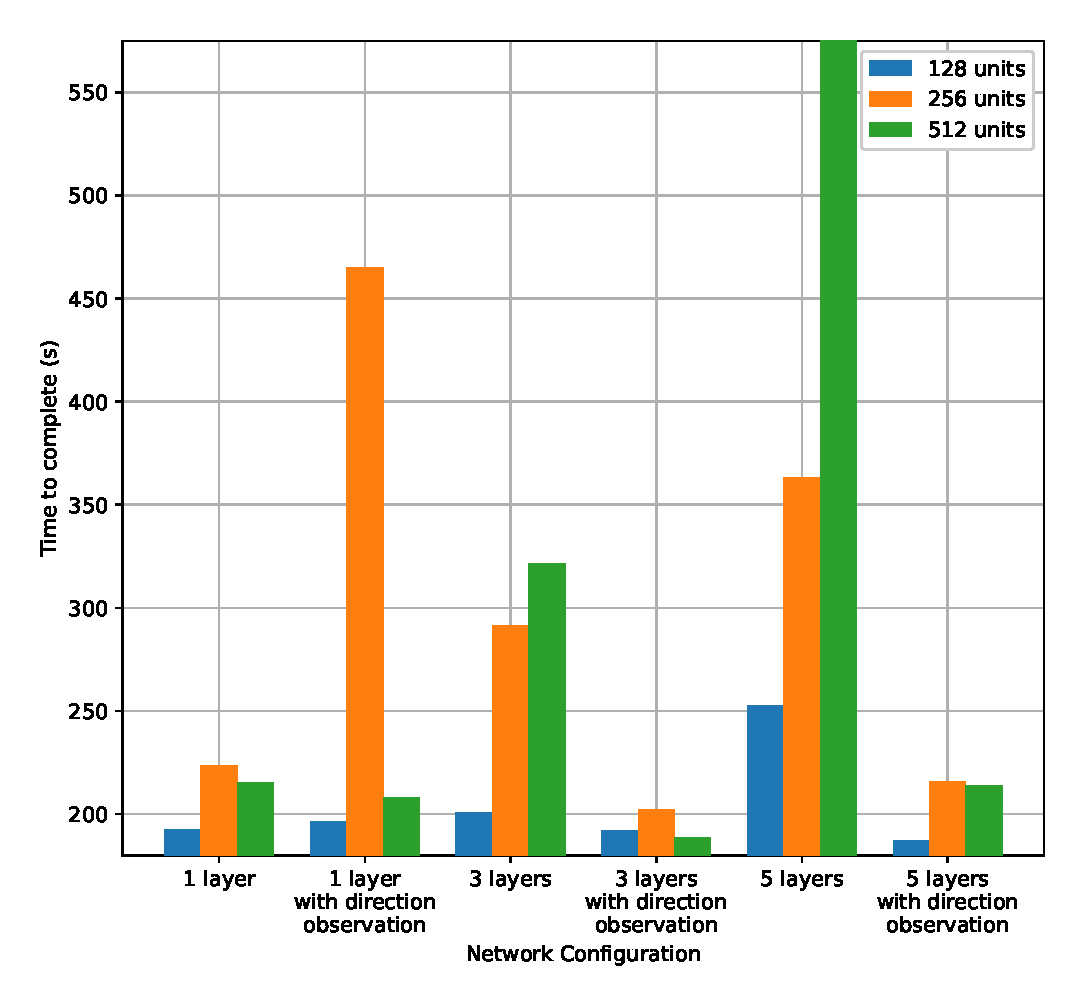
\includegraphics[width=\linewidth]{move_to_static_target_test_moving_brain_bar_chart.eps}
        \caption{Test results for reaching a static target using agent that was trained to reach moving targets}
        \label{test_results_static_target_moving_brain_bar_chart}
    \end{center}
\end{figure}


\subsection{Results comparasion}
Comparing the obtained results from the two approaches, the better one was when using an agent that was trained to reach static targets. The best time for this agent was 170.9822 seconds, while the best time obtained by the agent that was trained to reach moving targets was 187.1074 seconds, which is 16.1252 seconds slower ($8.61\%$). It is worth noting that both of these results came from architectures that had 5 hidden network layers and 128 units per layer.

The fact that the best result for reaching a static target was achieved by an agent that was trained to reach static targets is not surprising, since it was trained for this exact specific scenario.



\section{Reaching a moving target} \label{test_reach_moving_target}

For reaching a moving target, the test consists of an agent that has to touch 100 moving targets that appear in a predefined order and that have predefined paths that they will take. When a target appears it moves between predefined points using a predefined route, which is different for each of the 100 times the target appears. Once the agent reaches the target, the target appears at a different location, according to the predefined order, and the agent is reset to the middle of the level, so that it will start from the same place each times it chases a new target. This is done to make the test course be identical for each tested agent.

Just like in the previous section (\ref{test_reach_static_target}), the test will be run for both agents that were trained to reach moving targets and agents that were trained to reach static targets, and afterwards the results will be compared.


\subsection{Agent trained to reach moving targets}

The first ones to be tested will be the agents trained to reach moving targets. Both agents that do not observe the target's movement direction and agents that do are tested. The obtained results are in Table \ref{move_to_moving_target_test_results:2} and Figure \ref{test_results_moving_target_moving_brain_bar_chart}. 

For the architecture with a single hidden layer, the agents that did not observe the target's direction performed better than those that did, with the fastest configuration being the one with 512 units per layer, achieving a time of 452.052 seconds. It is followed by the configuration with 128 units, that was slower by 30.4473 seconds ($6.73\%$). The configuration with 256 units and that had the target's movement direction observation performed the worst out of all agents with a time of 688.592 seconds, over 3 minutes slower than the fastest configuration due to the fact that it took suboptimal paths when chasing the target and trying to avoid the objects in the environment in a weird manner.

Looking at the results for the architecture with 3 hidden layers, the agents that had the target's direction observation performed slightly better than the agents that did not have it. The best configuration is the one with 512 units per layer, which finished the course in 467.162 seconds. The configurations 128 and 256 units, with or without the extra observation, obtained similar results that were in the range of 484--491 seconds, which means that the difference between them was of at most $\sim1\%$. The configuration with 512 units that did not have the extra observation performed much worse, achieving a time of 602.9445 seconds, due to fact that it tried to avoid the objects placed in the level at a much greater distance than it should have.

The architecture with 5 hidden layers had very different results between the agents that used the target's movement direction observation and those that did not, whith the ones that did, performing much better, on average being faster by $\sim58$ seconds. The best configuration was the one with 128 units per layer, obtaining a time of 462.4213 seconds, with the other configurations lagging behind by over 38 seconds (at least $8.2\%$ slower).

\paragraph{}
In summary, it seems that the extra observation improves the agent's performance only when multiple hidden layers are used, otherwise it hinders its performance. The surprise here is that the fastest configuration had only one network layer, compared to the results from Section \ref{test_reach_static_target}, where the best results were obtained by agents that had a network with 5 hidden layers. Here, the difference between the best achieved time, form the agent with 1 hidden layer, and the second best time, from the agent with 5 hidden layers, is of 10.3693 seconds, which means that the second best agent was slower by $2.29\%$.

\begin{table}
    \centering
    \begin{tabular}{|| m{11.3em} | m{10em} | m{9.6em} ||}
    \hline \hline
    \strong{Network Configuration} & \strong{Observed target's direction} & \strong{Time to complete ($s$)} \\ \hline \hline
    1 layer, 128 units & No & 482.4993 \\ \hline
    1 layer, 128 units & Yes & 499.2063 \\ \hline
    1 layer, 256 units & No & 495.7267 \\ \hline
    1 layer, 256 units & Yes & 688.592 \\ \hline
    1 layer, 512 units & No & 452.052 \\ \hline
    1 layer, 512 units & Yes & 485.6294 \\ \hline
    3 layers, 128 units & No & 484.7428 \\ \hline
    3 layers, 128 units & Yes & 488.6792 \\ \hline
    3 layers, 256 units & No & 491.0297 \\ \hline
    3 layers, 256 units & Yes & 485.8719 \\ \hline
    3 layers, 512 units & No & 602.9445 \\ \hline
    3 layers, 512 units & Yes & 467.162 \\ \hline
    5 layers, 128 units & No & 527.4669 \\ \hline
    5 layers, 128 units & Yes & 462.4213 \\ \hline
    5 layers, 256 units & No & 549.7428 \\ \hline
    5 layers, 256 units & Yes & 500.7562 \\ \hline
    5 layers, 512 units & No & 568.0677 \\ \hline
    5 layers, 512 units & Yes & 506.722 \\ \hline \hline
    \end{tabular}
    \caption{Test results for reaching a moving target using agent that was trained to reach moving targets}
    \label{move_to_moving_target_test_results:2}
\end{table}

\begin{figure}
    \begin{center}
        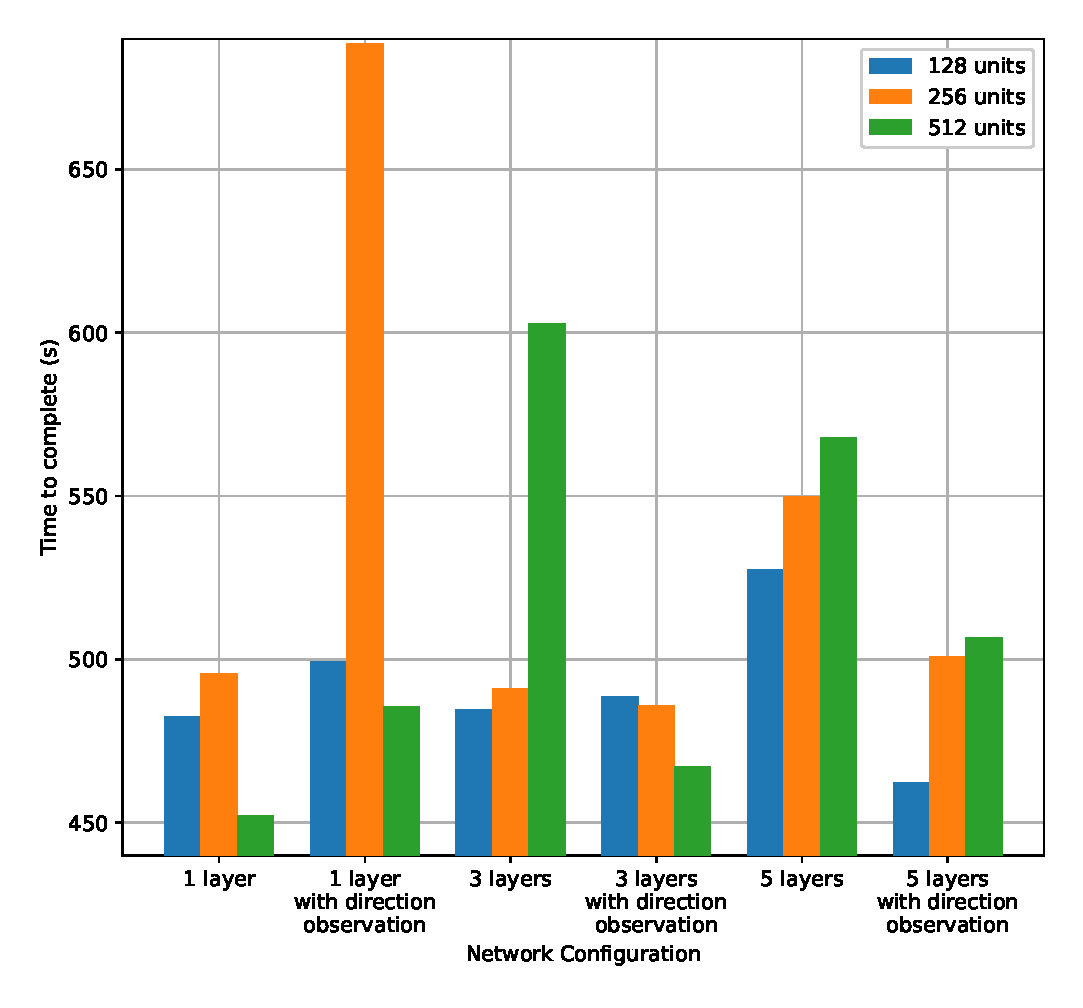
\includegraphics[width=\linewidth]{move_to_moving_target_test_moving_brain_bar_chart.eps}
        \caption{Test results for reaching a moving target using agent that was trained to reach moving targets}
        \label{test_results_moving_target_moving_brain_bar_chart}
    \end{center}
\end{figure}


\subsection{Agent trained to reach static targets}

Now, an agent that was trained to reach a static target will be tested to see how fast it will reach a moving target, and afterwards compare the results with the ones obtained by the agents that were trained to reach moving targets. The obtained results are in Table \ref{move_to_moving_target_test_results:2} and Figure \ref{test_results_moving_target_moving_brain_bar_chart}.

Looking at the results for the architecture with a single hidden layer, it can be seen that the best result, out of all the agents tested, is obtained by the one with the configuration with 128 units per layer, and which finishes the test course in 427.4408 seconds. The configuration with 256 units did not finish the course since it was unable to be trained. The configuration with 512 units is slower by 11.3486 seconds ($2.65\%$ slower).

For the architecture with 3 hidden layers, the configurations with 128 units and 512 units obtain results that are very similar, the only difference being of 1.8478 seconds ($0.41\%$), with the one with 512 units being the faster one. The configuration with 256 units is slightly slower, by 8.7071 seconds ($1.94\%$).

The architecture with 5 hidden layers has the second best performing agent, this being the one that has 128 units per layer and that finished the course in 429.3176 seconds. The other two agents managed to be slower, with the agent that had 256 units per layer being slower by 37.4474 seconds ($8.72\%$), and the agent that had 512 units being slower by 33.408 seconds ($7.78\%$).

The architecture with 7 layers, has the slowest results, with the best one from this architecture being the configuration with 128 units which managed to finish the test in 465.1996 seconds. The slowest configuration was the one that had 512 units per layer, finishing the course in 546.0353 seconds, $17.37\%$ slower than the one with 128 units. Again, the agent tries to make very large turns to avoid other objects, which make him lose a lot of time.

\paragraph{}
In summary, the best agent was the one that had an architecture with 1 hidden layer and 128 units per layer, finishing the test in 427.4408 seconds, and being closely followed by the agent with the architecture with 5 hidden layers and 128 units, which was slower by 1.8768 seconds. This shows, that unlike the test in Section \ref{test_reach_static_target}, having a smaller network leads to better results.

\begin{table}
    \centering
    \begin{tabular}{|| m{15em} | m{15em} ||}
    \hline \hline
    \strong{Network Configuration} & \strong{Time to complete ($s$)} \\ \hline \hline
    1 layer, 128 units & 427.4408 \\ \hline
    1 layer, 256 units & DNF \\ \hline
    1 layer, 512 units & 438.7894 \\ \hline
    3 layers, 128 units & 450.3436 \\ \hline
    3 layers, 256 units & 457.2029 \\ \hline
    3 layers, 512 units & 448.4958 \\ \hline
    5 layers, 128 units & 429.3176 \\ \hline
    5 layers, 256 units & 466.765 \\ \hline
    5 layers, 512 units & 462.7256 \\ \hline
    7 layers, 128 units & 465.1996 \\ \hline
    7 layers, 256 units & 479.0871 \\ \hline
    7 layers, 512 units & 546.0353 \\ \hline \hline
    \end{tabular}
    \caption{Test results for reaching a moving target using agent that was trained to reach static targets}
    \label{move_to_moving_target_test_results:1}
\end{table}

\begin{figure}
    \begin{center}
        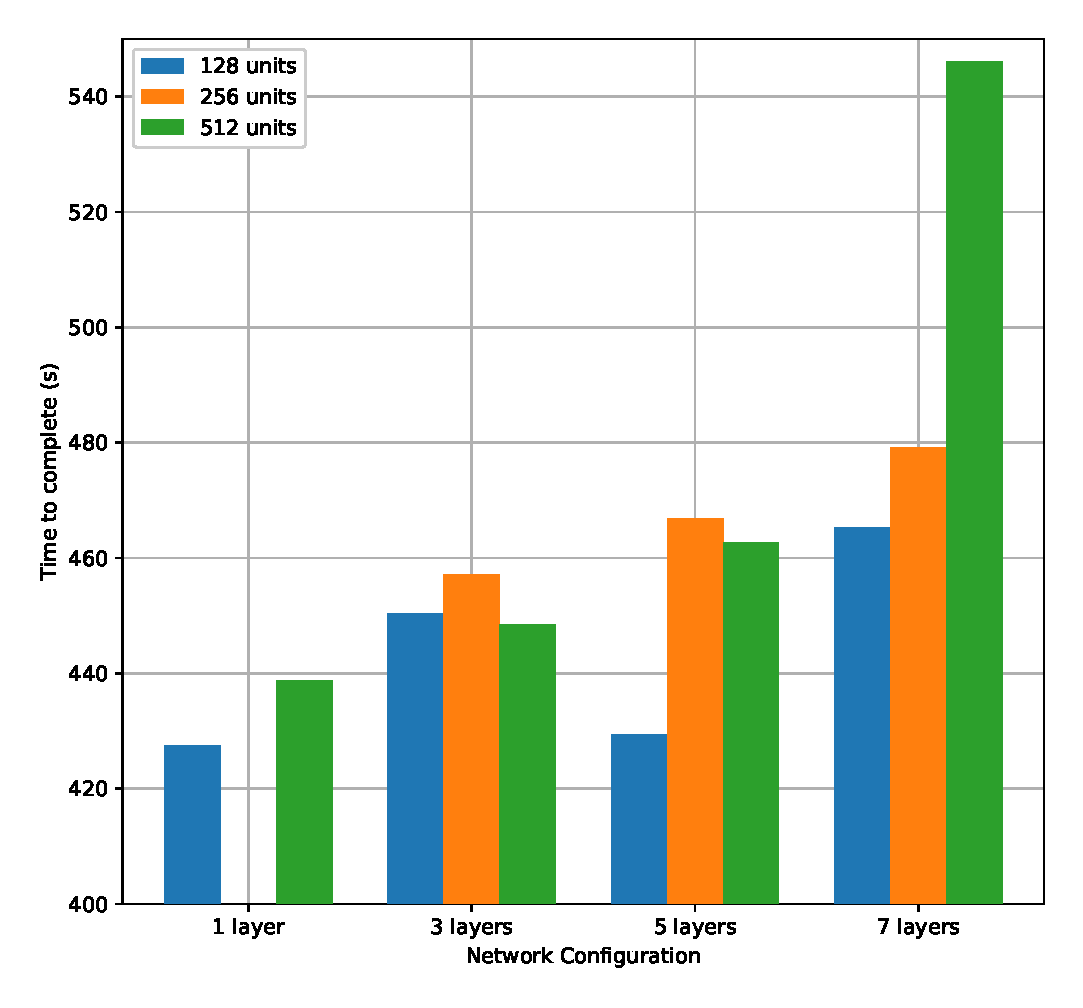
\includegraphics[width=\linewidth]{move_to_moving_target_test_static_brain_bar_chart.eps}
        \caption{Test results for reaching a moving target using agent that was trained to reach static targets}
        \label{test_results_moving_target_static_brain_bar_chart}
    \end{center}
\end{figure}

\subsection{Results comparasion}
Comparing the obtained results, it can be seen that the agent who was trained to reach static targets, performs better than the agent trained to reach moving targets. The fastest agent trained to reach static targets finished the test in 427.4408 seconds, while the fastest agent trained to reach moving targets finished the test in 452.052 seconds, being slower by 24.6112 seconds ($5.75\%$). This means that training an agent for a particular task could make it perform a more advanced version of that task better than an agent trained specifically for that advanced task. It is also worth noting that both agents had a network with a single hidden layer.


\section{Shooting a moving target} \label{test_shoot_moving_target}

For shooting a moving target, the test is built just like it is described in Section \ref{test_reach_moving_target}, the only difference being that the agent is not supposed to reach the target, but to shoot it. The two types of trained agents will be tested, however, comparasions between them regarding how fast can they finish the test are not as important as before, since one of the approaches is supposed to be more aggressive (the \emph{naive} one), and the other is supposed to be more defensive (the tactical one), with the result being that the more aggressive apporach should finish the test faster.

\subsection{Agent trained in a \emph{naive} manner}

For the \emph{naive} approach, the results can be seen in Table \ref{shoot_moving_targets_test_results:1} and Figure \ref{test_results_shoot_moving_target_bar_chart}. The architecture with a single hidden layer obtained the best results with the configuration that has 128 units per layer obtaining the best result, which is 499.8927 seconds. The configuration with 256 units was slower by 64.8033 seconds ($12.96\%$), while the one with 512 units per layer was slower by 36.7426 seconds ($7.35\%$).

For the architecture with 3 hidden layers, the configuration 128 units per layer was agian the fastest one, managing to finish the test in 590.7621 seconds, however it was slower than any of the configurations with a single hidden layer. The configuration with 256 units was slower by 46.3229 seconds ($7.84\%$), while the one with 512 units was slower by 145.5966 seconds ($24.64\%$) which is a significant increase.

Looking at the results for the architecture with 5 hidden layers, it can be observed that, again, the best configuration is the one with 128 units per layer, with a time of 606.5751 seconds. The configuration with 256 units was slower by 68.4348 seconds ($11.28\%$), while the configuration with 512 units was slower by 211.0569 seconds ($34.79\%$), which is a big increase in the time to finish the test.

The architecture with 7 layers, has the slowest results out of all the architectures, with the configuration with 128 units per layer obtaining a time of 837.6456 seconds, which is slower than any of the other architectures. The configuration with 256 units per layer is slower by 34.5383 seconds ($4.12\%$), while the one with 512 units is slower by 76.8397 seconds ($9.17\%$).

\paragraph{}
In summary, the fastest architectures were the ones that had only 128 units per layer, with the fastest one being the one with a single hidden layer and which finished the test in 499.8927 seconds. The slowest architectures were the ones with 512 units per layer, with the slowest one being the one with 7 hidden layer and which finished the test in 914.4853 seconds, taking almost twice as much time as the fastest agent. It is worth noting that increasing the number of hidden layers and also the number of units per layer, is alost guaranteed to decrease the performance of the agent.

\begin{table}
    \centering
    \begin{tabular}{|| m{15em} | m{15em} ||}
    \hline \hline
    \strong{Network Configuration} & \strong{Time to complete ($s$)} \\ \hline \hline
    1 layer, 128 units & 499.8927 \\ \hline
    1 layer, 256 units & 564.696 \\ \hline
    1 layer, 512 units & 536.6353 \\ \hline
    3 layers, 128 units & 590.7621 \\ \hline
    3 layers, 256 units & 637.085 \\ \hline
    3 layers, 512 units & 736.3587 \\ \hline
    5 layers, 128 units & 606.5751 \\ \hline
    5 layers, 256 units & 675.0099 \\ \hline
    5 layers, 512 units & 817.632 \\ \hline
    7 layers, 128 units & 837.6456 \\ \hline
    7 layers, 256 units & 872.1839 \\ \hline
    7 layers, 512 units & 914.4853 \\ \hline \hline
    \end{tabular}
    \caption{Test results for shooting a moving target using agent that was trained using \emph{naive} method}
    \label{shoot_moving_targets_test_results:1}
\end{table}

\begin{figure}
    \begin{center}
        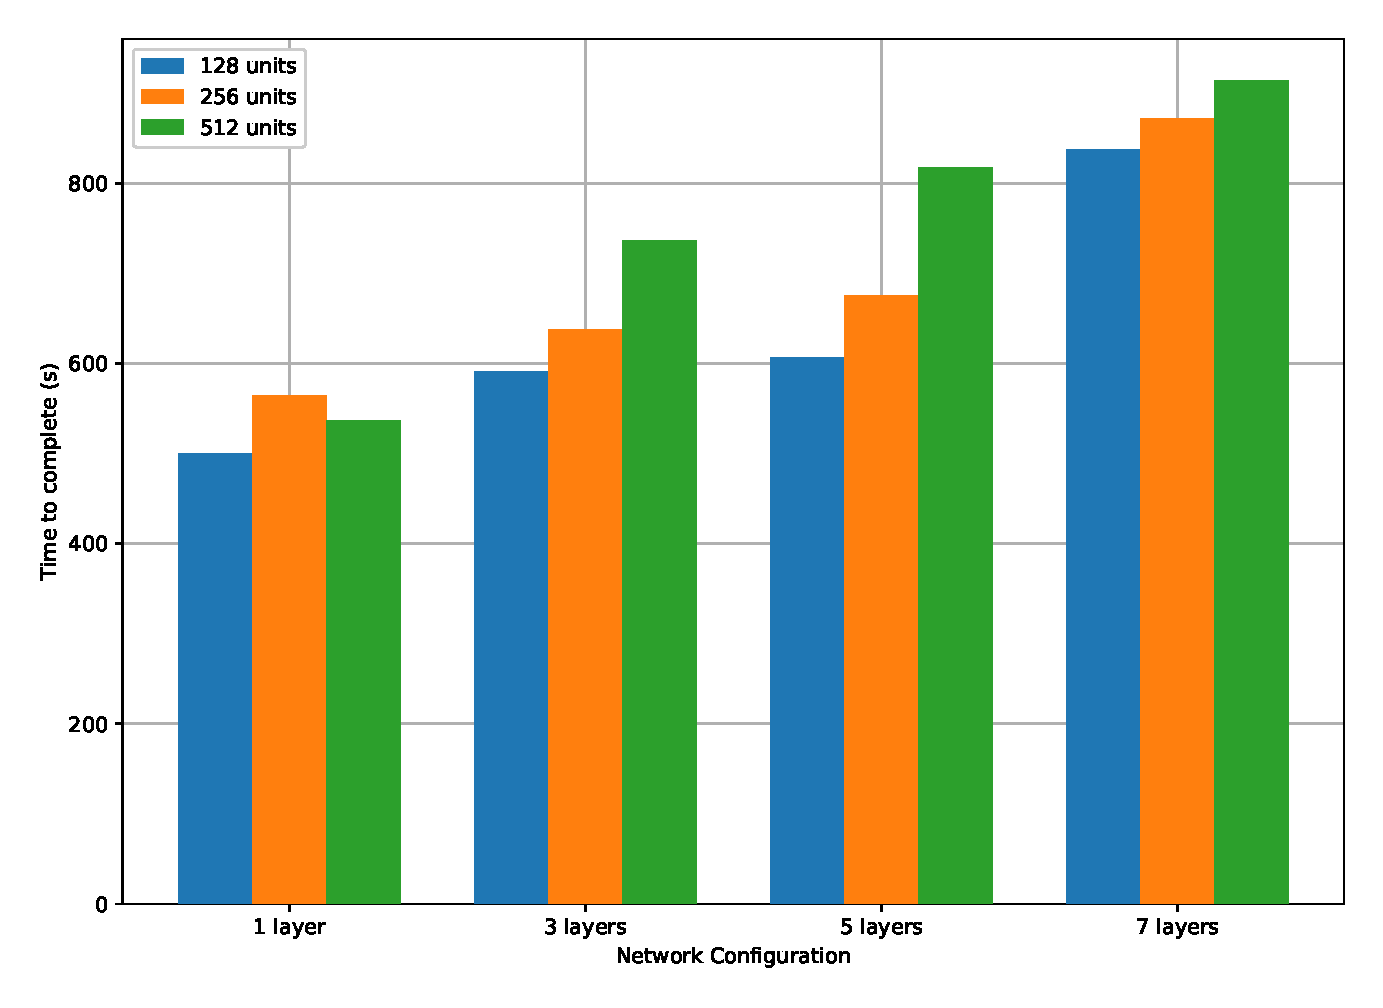
\includegraphics[width=\linewidth]{shoot_moving_target_test_bar_chart.eps}
        \caption{Test results for shooting a moving target using agent that was trained using \emph{naive} method}
        \label{test_results_shoot_moving_target_bar_chart}
    \end{center}
\end{figure}



\paragraph{}
Just like in Section \ref{subsubsection:shoot_naive}, there will be a comparasion between the results obtained when changing the bullet observations. Each agent will have an architecture with a certain number of hidden layers and 128 units per layer. The observation combinations are the following:
\begin{itemize}
    \item Bullet's trajectory and speed, and if the bullet was fired
    \item Bullet's speed and if the bullet was fired
    \item Only if the bullet was fired
\end{itemize}

The test results can be seen in Table \ref{shoot_moving_targets_test_results:2} and Figure \ref{test_results_shoot_moving_target_obs_comparasion_bar_chart}. For the architecture with a single hidden layer, the fastest resultis obtained by the agent that observers only if the bullet was fired, finishing the test in 499.8927 seconds. In the second place is the agent that makes all three observations about the bullet, being slower by 28.301 seconds ($5.66\%$), and in the third place is the agent that makes two observations about the bullet, and it's slower by 47.3781 seconds ($9.47\%$).

For the architecture with 3 hidden layers, the fastest agent is the one that makes all thee observations regarding the bullet, and finishes the test in 529.0487 seconds, almost identical to the performance achieved by the same type of agent, but with a network with a single hidden layer. It is followed by the agent that make two observations regarding the bullet, being slower by 28.5645 seconds ($5.39\%$), and finally, by the agent that only observes if the bullet is fired, being slower by 61.7134 seconds ($11.66\%$).

The architecture with 5 hidden layers, again, has the the fastest agent being the one that observes only if the bullet was fired, and the agent finishes the test in 606.5751 seconds. It is closely followed by the agent that used all three bullet observations, being slower by 22.0864 seconds ($3.64\%$), and then by the agent with two bullet observations, which was slower by 81.5199 seconds ($13.43\%$).

Looking at the results for the architecture with 7 hidden layers, the agents that had 2 or 3 observations regarding the bullet performed virtually identically, having a difference of only 2.4008 seconds, while the agent that observed only if the bullet was fired was slower by 152.7139 seconds ($22.29\%$).

\paragraph{}
In summary, it can be seen that increasing the number of layers also makes the agent perfrom more poorly, with the agents that had a network architecture witha  single hidden layer performing the best. It can aslo be observed that when the number of layers is lower, it is best not to include additional observations regarding the bullet and only keep the one that tells if the bullet was fired.

\begin{table}
    \centering
    \begin{tabular}{|| m{11.5em} | m{13em} | m{10em} ||}
    \hline \hline
    \strong{Network Configuration} & \strong{Bullet Observations} & \strong{Time to complete ($s$)} \\ \hline \hline
    1 layer, 128 units & Bullet's trajectory and speed & 528.1937 \\ \hline
    1 layer, 128 units & Bullet's speed & 547.2708 \\ \hline
    1 layer, 128 units & Only if bullet was fired & 499.8927 \\ \hline
    3 layers, 128 units & Bullet's trajectory and speed & 529.0487 \\ \hline
    3 layers, 128 units & Bullet's speed & 557.6132 \\ \hline
    3 layers, 128 units & Only if bullet was fired & 590.7621 \\ \hline
    5 layers, 128 units & Bullet's trajectory and speed & 628.6615 \\ \hline
    5 layers, 128 units & Bullet's speed & 688.095 \\ \hline
    5 layers, 128 units & Only if bullet was fired & 606.5751 \\ \hline
    7 layers, 128 units & Bullet's trajectory and speed & 687.3325 \\ \hline
    7 layers, 128 units & Bullet's speed & 684.9317 \\ \hline
    7 layers, 128 units & Only if bullet was fired & 837.6456 \\ \hline \hline
    \end{tabular}
    \caption{Test results for shooting a moving target using agent that was trained using \emph{naive} method and different bullet observation combinations}
    \label{shoot_moving_targets_test_results:2}
\end{table}

\begin{figure}
    \begin{center}
        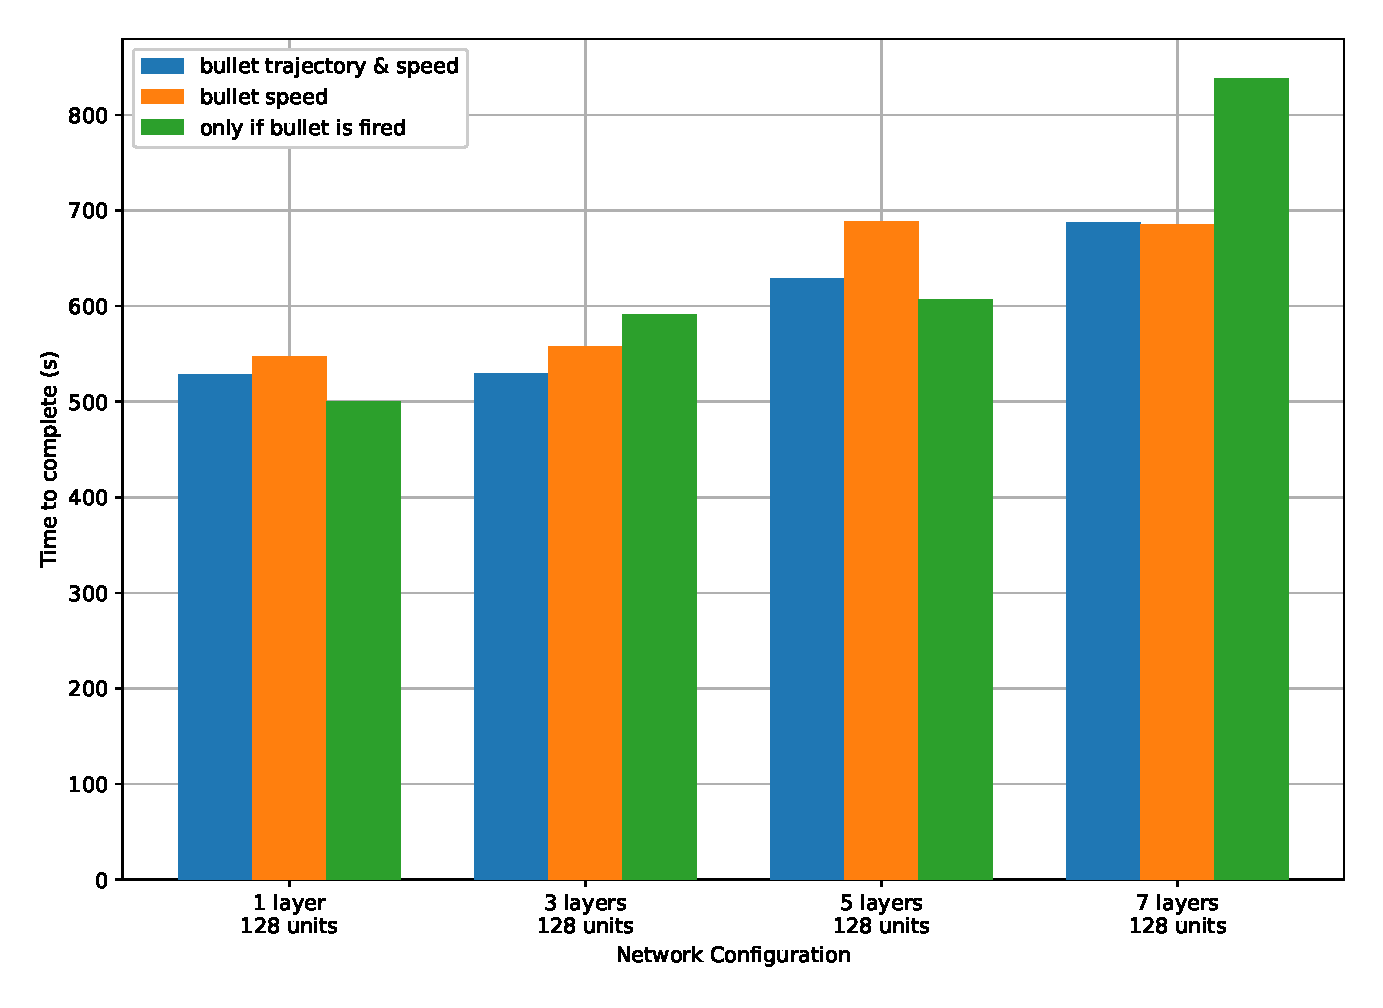
\includegraphics[width=\linewidth]{shoot_moving_target_test_obs_comparasion_bar_chart.eps}
        \caption{Test results for shooting a moving target using agent that was trained using \emph{naive} method and different bullet observation combinations}
        \label{test_results_shoot_moving_target_obs_comparasion_bar_chart}
    \end{center}
\end{figure}


\subsection{Agent trained in a tactical manner}


\begin{table}
    \centering
    \begin{tabular}{|| m{15em} | m{15em} ||}
    \hline \hline
    \strong{Network Configuration} & \strong{Time to complete ($s$)} \\ \hline \hline
    1 layer, 128 units & 605.0273 \\ \hline
    1 layer, 256 units & 483.9203 \\ \hline
    1 layer, 512 units & 494.5686 \\ \hline
    3 layers, 128 units & 590.4073 \\ \hline
    3 layers, 256 units & 679.4313 \\ \hline
    3 layers, 512 units & 762.0126 \\ \hline
    5 layers, 128 units & 650.9454 \\ \hline
    5 layers, 256 units & 701.7521 \\ \hline
    5 layers, 512 units & 1528.791 \\ \hline
    7 layers, 128 units & 687.3971 \\ \hline
    7 layers, 256 units & 937.4277 \\ \hline
    7 layers, 512 units & 2200.825 \\ \hline \hline
    \end{tabular}
    \caption{Test results for shooting a moving target using agent that was trained using tactical method}
    \label{shoot_moving_targets_v2_test_results:1}
\end{table}

\begin{figure}
    \begin{center}
        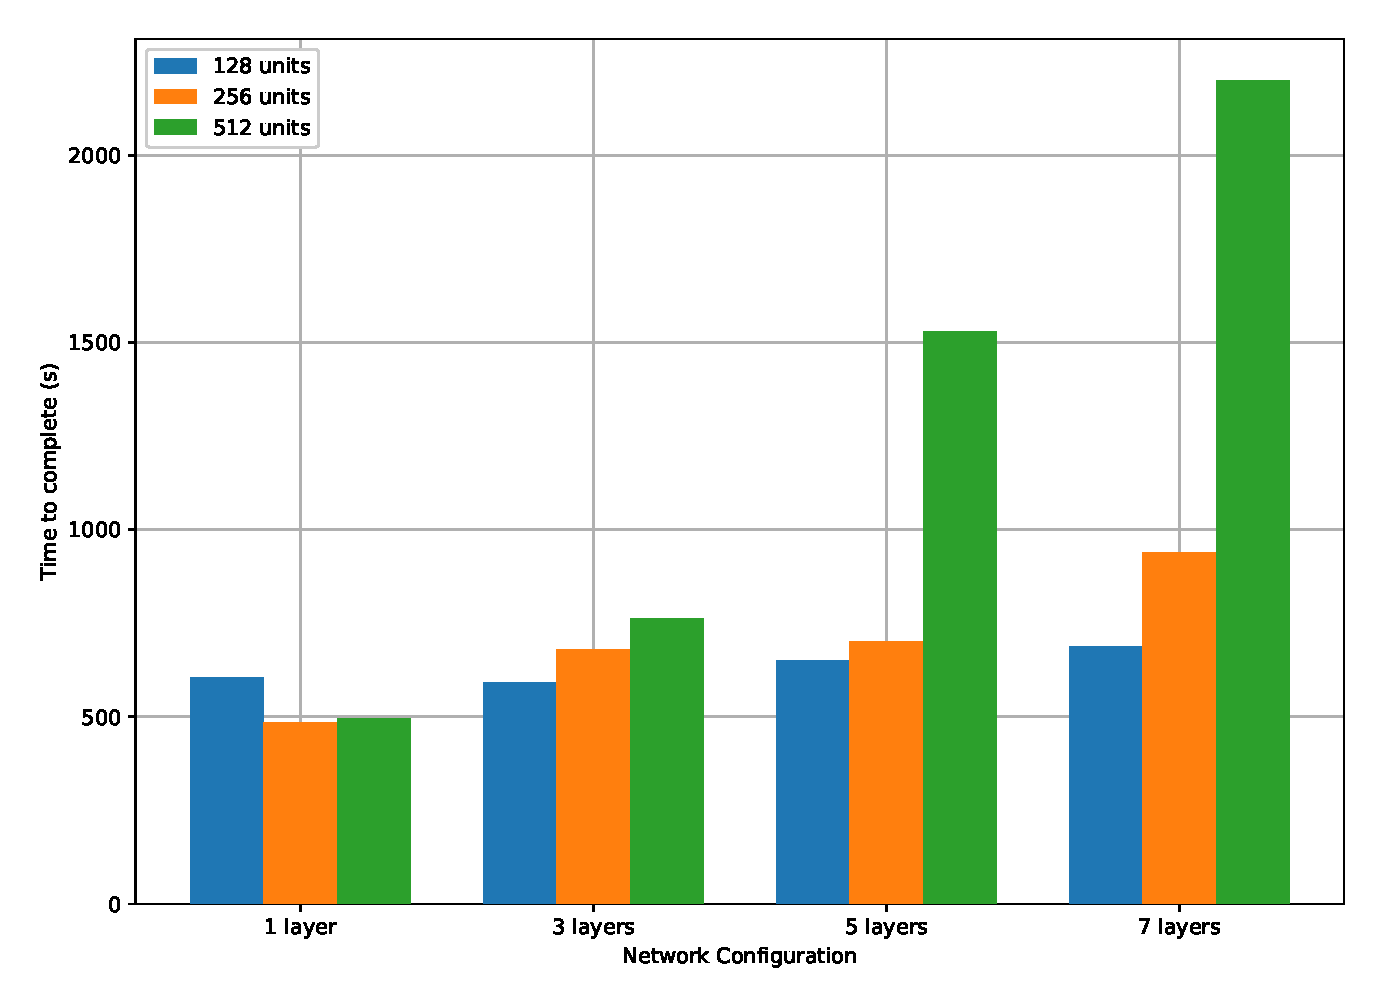
\includegraphics[width=\linewidth]{shoot_moving_target_v2_test_bar_chart.eps}
        \caption{Test results for shooting a moving target using agent that was trained using tactical method}
        \label{test_results_shoot_moving_target_v2_bar_chart}
    \end{center}
\end{figure}


\section{Fighting against an AI controlled enemy}

TODO: sa fac sa pot sa bat un tank, dupa sa vad daca paote sa bata inamicu, si daca da, sa vad cat de repede poa sa bata inamicu de x ori (eventual sa fac un mean time per round, sau sa zic de cate ori a fost lovit, etc)